\documentclass{article}
\usepackage{graphicx} % Required for inserting images

\title{GIT}
\author{Idriss BADO}
\date{January 2025}

\begin{document}

\maketitle

\section*{Git Commands for the assessment}



Below is the sequence of Git commands to follow:

\begin{verbatim}
Step 1: Create a folder called learn_git
mkdir learn_git

Step 2: Change directory into the learn_git folder
cd learn_git

Step 3: Create a file called third.txt
touch third.txt

Step 4: Initialize an empty git repository
git init

Step 5: Add third.txt to the staging area
git add third.txt

Step 6: Commit with the message "adding third.txt"
git commit -m "adding third.txt"

Step 7: Check out your commit with git log
git log

Step 8: Create another file called fourth.txt
touch fourth.txt

Step 9: Add fourth.txt to the staging area
git add fourth.txt

Step 10: Commit with the message "adding fourth.txt"
git commit -m "adding fourth.txt"

Step 11: Remove the third.txt file
rm third.txt

Step 12: Add this change to the staging area (removal of third.txt)
git add .

Step 13: Commit with the message "removing third.txt"
git commit -m "removing third.txt"

Step 14: Check out your commits using git log
git log

Step 15: Change your global settings to core.pager=cat
git config --global core.pager "cat"

Step 16: List all global configurations for git
git config --global --list
\end{verbatim}
Here is a screenshot of the work i have completed in the terminal:
\begin{figure}[h!]
    \centering
    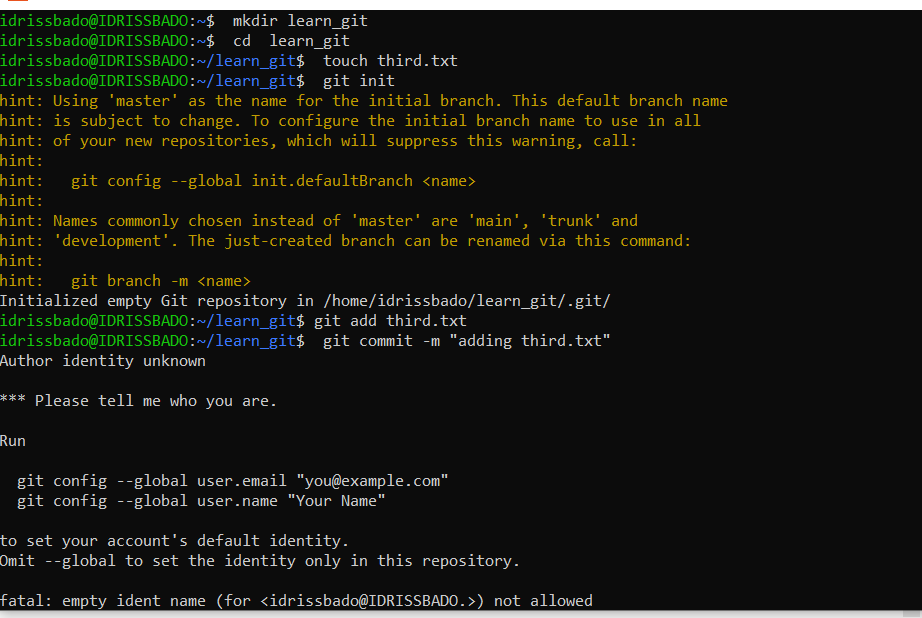
\includegraphics[width=1.4\textwidth]{idriss1.PNG}  
    \caption{Screenshot of the terminal commands executed.}
    \label{fig:screenshot}
\end{figure}
\begin{figure}[h!]
    \centering
    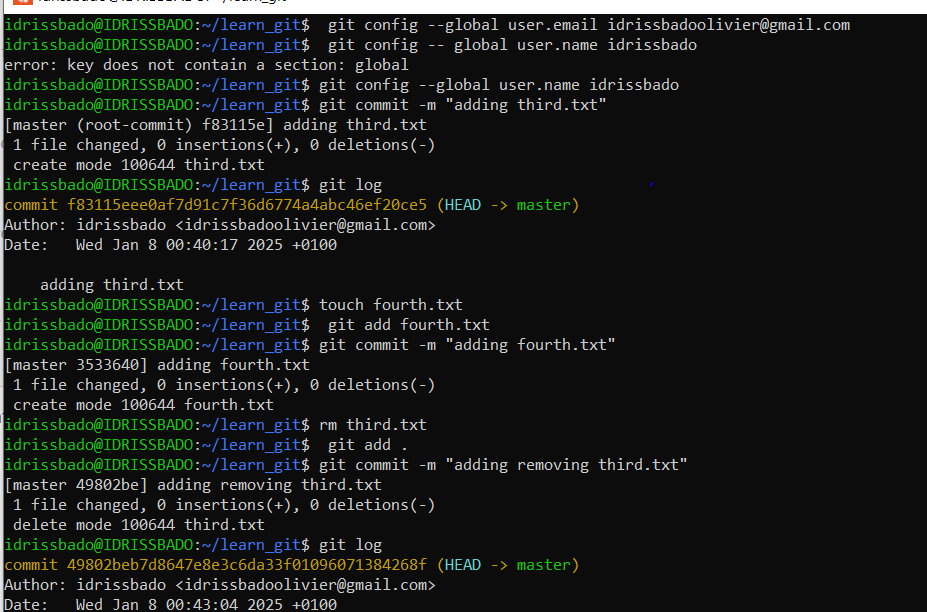
\includegraphics[width=1.4\textwidth]{IDRISS2.PNG} 
    \caption{Screenshot of the terminal commands executed.}
    \label{fig:screenshot}
\end{figure}
\begin{figure}[h!]
    \centering
    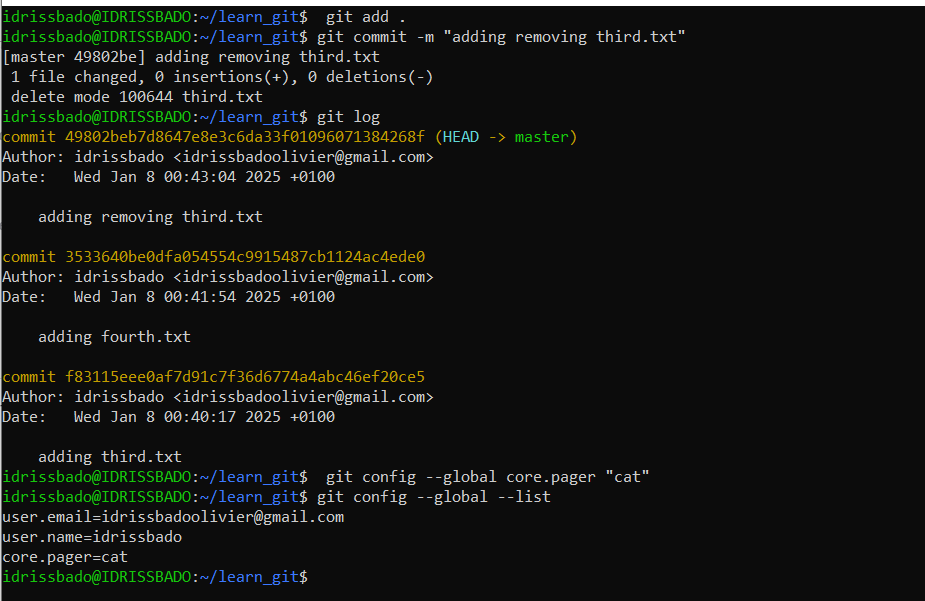
\includegraphics[width=1.4\textwidth]{IDRISS3.PNG} 
    \caption{Screenshot of the terminal commands executed.}
    \label{fig:screenshot}
\end{figure}
\end{document}
